\documentclass[a4paper]{refart}

\usepackage[utf8]{inputenc}
\usepackage[T1]{fontenc}
\usepackage[osf,sc]{mathpazo}
\usepackage{hyperref}
\usepackage[english,nameinlink]{cleveref}
\usepackage{microtype}
\usepackage{figlatex}
\usepackage{textcomp}
\usepackage{amsmath}
\usepackage{tocloft}
\usepackage{xspace}
\usepackage{cite}

\hypersetup{
  bookmarksdepth=2,
  bookmarksnumbered=true,
  bookmarksopen=true,
  bookmarksopenlevel=2,
  colorlinks=true,
  linktocpage=true,
  breaklinks=true,
  pageanchor=true,
  allcolors=[rgb]{0.7,0.1,0.1},
  pdftitle={The Cunf Tool User's Manual, v1.6.1},
  pdfauthor={Cesar Rodriguez}
}

%\newcommand\acq		{\mathsf{P}}
%\newcommand\comp	{\mathfrak{c}}
%\newcommand\cycles[1]	{\mathsf{Cycles}{(#1)}}
%\newcommand\eager[1]	{\mathsf{Eager}{(#1)}}
%\newcommand\eenr	{\mathcal{E}}
%\newcommand\enr[1]	{\mathcal{E}_{#1}}
%\newcommand\extens[1]	{\mathsf{Extensions }(#1)}
%\newcommand\extn	{\mathcal{X}}
%\newcommand\lazy[1]	{\mathsf{Lazy}{(#1)}}
%\newcommand\lchist[2]	{{ {#1}\langle#2\rangle }}
%\newcommand\lonepref	{\ppref^1_{N}}
%\newcommand\lpg		{\leadsto_\config}
%\newcommand\lstruc	{\mathcal{L}}
%\newcommand\ltwopref	{\ppref^2_{N}}
%\newcommand\maxspoilers[1]{t^{\spoils}_{#1}}
%\newcommand\move[1]	{\stackrel{#1}{\longrightarrow }}
%\newcommand\myleq	\le
%\newcommand\nat		{\mathrm{I\!N}}
%\newcommand\node[1]	{\mathit{#1}}
%\newcommand\pac		{\mathrel{\nearrow\!\!\!\!\!\nearrow}}
%\newcommand\rd		\propto
%\newcommand\spoils	{\dagger}

% relations
\newcommand\reveals	{\mathrel{\triangleright}}
\newcommand\ac		{\mathrel{\nearrow}}
\newcommand\aco		{\mathrel{/\!/}}
\newcommand\cfl		{\mathrel{\#}}
\newcommand\co		{\mathrel{\parallel}}
\newcommand\eqdef	{\mathrel{:=}}
\newcommand\evolves	{\mathrel{\sqsubseteq}}
\newcommand\evstrict	{\mathrel{\sqsubset}}
\newcommand\ispref	{\mathrel{\preceq}}
\newcommand\icause	{\mathrel{<_i}}
\newcommand\ifft	{\mathrel{\text{ iff }}}
\newcommand\nco		{\mathrel{\not\!\!\;\,\co}}

\newcommand\extreveals	{\mathbin{-\hspace{-2.5mm}-\hspace{-2.0mm}\reveals}}

% operators
\newcommand\merge[1]	{\mathop{\mathfrak{Merge}} (#1)}
\newcommand\od[1]	{\mathop{\mathrm{od}} (#1)}
\newcommand\amo[1]	{\mathop{\text{AMO}} (#1)}
\newcommand\bigo[1]	{\mathop{\mathcal{O}} (#1)}
\newcommand\progloop[1]	{\mathop{\mathit{ploop}} (#1)}
\newcommand\allhist[1]	{\mathop{\mathit{Hist}} (#1)}
\newcommand\compt[1]	{\mathop{\mathit{compat}} (#1)}
\newcommand\conc[1]	{\mathop{\mathit{conc}} (#1)}
\newcommand\conf[1]	{\mathop{\mathit{conf}} (#1)}
\newcommand\cut[1]	{\mathop{\mathit{cut}} (#1)}
\newcommand\explain[1]	{\mathop{\mathit{expl}} (#1)}
\newcommand\lpo[1]	{\mathop{\mathit{lpo}} (#1)}
\newcommand\marking[1]	{\mathop{\mathit{mark}} (#1)}
\newcommand\obser[1]	{\mathop{\mathit{obs}} (#1)}
\newcommand\peel[2]	{\mathop{\mathit{peel}}_{#2} (#1)}
\newcommand\peelast[1]	{\mathop{\mathit{peel}}^* (#1)}
\newcommand\reach[1]	{\mathop{\mathit{reach}} (#1)}
\newcommand\runs[1]	{\mathop{\mathit{runs}} (#1)}
\newcommand\sfp[1]	{\mathop{\mathit{pred}} (#1)}
\newcommand\spoilers[1]	{\mathop{\mathit{spoilers}} (#1)}
\newcommand\state[1]	{\mathop{\mathit{state}} (#1)}
\newcommand\succexpl[1]	{\mathop{\mathit{succexpl}} (#1)}
\newcommand\trim[2]	{\mathop{\mathit{trim}_{#2}} (#1)}
\newcommand\trimast[1]	{\mathop{\mathit{trim}}^* (#1)}
\newcommand\depth[1]	{\mathop{\mathit{depth}} (#1)}

\newcommand\sem[1]	{\mathrm{[\![{#1}]\!]}}
\newcommand\hist[2]	{{ {#1}[\![#2]\!] }}
\newcommand\cont[1]	{\underline{#1}}
\newcommand\post[1]	{#1^\bullet}
\newcommand\pre[1]	{{}^\bullet#1}
\newcommand\support[1]	{\bar{#1}}

\newcommand\FIXME[1]	{\texttt{FIXME: #1}}
\newcommand\anc[1]	{{#1}^\uparrow}
\newcommand\unf[1]	{\mathcal{U}_{#1}}
\newcommand\unr[1]	{\mathcal{M}_{#1}}
\newcommand\var[1]	{\mathsf{#1}}
\newcommand\mer[1]	{\mathcal{Q}_{#1}}
\newcommand\hst[1]	{\mathcal{H}_{#1}}
\newcommand\trunc[1]	{\mathcal{T}_{#1}}
\newcommand\htrunc[1]	{\widehat{\mathcal{T}}_{#1}}
\newcommand\pref[1]	{\mathcal{P}_{#1}}

% abbreviations
\newcommand\precutoff	{\text{$\prec$-cutoff}}
\newcommand\phiasym	{\phi_{\ppref}^\text{asym}}
\newcommand\phicausal	{\phi_{\ppref}^\text{causal}}
\newcommand\phidead	{\phi_{\ppref}^\text{dead}}
\newcommand\phidis	{\phi_{\ppref}^\text{dis}}
\newcommand\phimark	{\phi_{\ppref}^\text{mark}}
\newcommand\phip	{\phi_{\ppref}}
\newcommand\phisym	{\phi_{\ppref}^\text{sym}}
\newcommand\mcitomp	{\textsc{Mci2mp}\@\xspace}
\newcommand\minisat	{\textsc{MiniSat}\@\xspace}
\newcommand\mole	{\textsc{Mole}\@\xspace}
\newcommand\prcompress	{\textsc{PRCompress}\@\xspace}
\newcommand\clp		{\textsc{Clp}\@\xspace}
\newcommand\cmerge	{\textsc{Cmerge}\@\xspace}
\newcommand\cunf	{\textsc{Cunf}\@\xspace}
\newcommand\cosyverif	{\textsc{Cosyverif}\@\xspace}
\newcommand\coloane	{\textsc{Coloane}\@\xspace}
\newcommand\tapaal	{\textsc{Tapaal}\@\xspace}
\newcommand\cunft	{Cunf~Tool}
\newcommand\cna		{\textsc{Cna}\@\xspace}
\newcommand\punf	{\textsc{Punf}\@\xspace}
\newcommand\salpha	{\ppref_\alpha}
\newcommand\spcutoff	{\text{sp-cutoff}}
\newcommand\id		{\textit{id}}
\newcommand\cep		{EP}

\newcommand\ppref	{\mathcal{P}}
\newcommand\qpref	{\mathcal{Q}}
\newcommand\con		{\mathcal{C}}
\newcommand\N		{\mathbb{N}}
\newcommand\Q		{\mathbb{Q}}
\newcommand\R		{\mathbb{R}}
\newcommand\obs		{\mathbb{O}}
\newcommand\hhat	{\widehat h}
\newcommand\ehat	{\widehat e}
\newcommand\chat	{\widehat c}
\newcommand\Cohat	{\widehat \con}
\newcommand\Hihat	{\widehat H}

\newcommand\pp		{pp.\@\xspace}
\newcommand\viz		{viz.\@\xspace}
\newcommand\vs		{vs.\@\xspace}
\newcommand\wlogg	{w.l.o.g.,\xspace}
\newcommand\aka		{a.k.a.\xspace}
\newcommand\wrt		{w.r.t.\@\xspace}
\newcommand\cf		{cf.\@\xspace}
\newcommand\Wlog	{W.l.o.g.,\xspace}
\newcommand\al		{al.\@\xspace}
\newcommand\eg		{e.g.\@\xspace}
\newcommand\etc		{etc.\@\xspace}
\newcommand\ie		{i.e.\@\xspace}
\newcommand\naive	{na{\"\i}ve\xspace}

% miscellaneous
\newcommand\cod[1]	{\texttt{#1}}
\newcommand\tup[1]	{\langle#1\rangle}
\newcommand\set[1]	{{\{ \, #1 \, \mathclose \}}}
\newcommand\eqtag[1]	{\hfill{} \refstepcounter{equation} \label{#1} (\arabic{equation})}

\newtheorem{cor}	{Corollary}
\newtheorem{defn}	{Definition}
\newtheorem{lemma}	{Lemma}
\newtheorem{prop}	{Proposition}
\newtheorem{remark}	{Remark}
\newtheorem{theorem}	{Theorem}

% a  appendix
% c  chapter
% o  corollary
% d  def
% e  equation
% f  figure
% l  lemma
% p  proposition
% r  remark
% s  section
% t  table
% h  theorem



\title{The \cunft{} User's Manual \hfill v1.6.1}
\author{C\'esar Rodr\'iguez}
%\date{April 2013}

\begin{document}
\maketitle

\begin{abstract}
This is both a user guide and a tutorial of the \cunft{}.
The \cunft{} is a toolset for carrying out unfolding-based
verification of Petri nets extended with read arcs, also called
\emph{contextual nets} (c-nets).
Unfoldings fully represent the state-space (reachable markings) of a c-net
by a partial order rather than by a set of interleavings;
they are often exponentially smaller than the reachablity graph, and never
larger than it.
Additionally, c-net unfoldings can be exponentially more compact than
those of corresponding Petri nets.
The toolset specifically contains one unfolding-construction
tool and one reachablity and deadlock-checking tool.
\end{abstract}

\tableofcontents

\section{Introduction}%{{{
\label{s:intro}

The \emph{\cunft{}} is a \emph{set}
of programs for carrying out unfolding-based
verification of Petri nets extended with read arcs, \aka contextual
nets, or c-nets.  The package specifically contains the following tools:
\begin{enumerate}
\item
  \cunf: constructs the unfolding of a c-net;
\item
  \cna: performs reachability and deadlock analysis using unfoldings
  constructed by \cunf.
\item
  Scripts such as \verb!pep2dot! or \verb!grml2pep! to do format conversion
  between various Petri net formats, unfolding formats, \etc
\end{enumerate}

Petri nets are a modelling language for concurrent systems.
The reader unfamiliar to the topic could perhaps start with\cite{wiki:pn}
or\cite{Mur89}.

Contextual nets are Petri nets where, in addition to the ordinary
\textit{arrows} between places and transitions, one may find
\emph{read arcs}.
These allow transitions to verify that
tokens exist in a place before firing, but don't consume them
when firing.
Transitions can then be thought of reading a
\emph{context} required to fire, hence the name.
See Section~2 of\cite{BBCKRS12} for a brief formalization
and\cite{MR95} for more details.
% FIXME example before saying formalization

Observe that every Petri net is a contextual net (without read arcs).
Also notice that for every c-net we obtain an equivalent Petri net after
substituting read arcs for pairs of \emph{consume-produce} loops.  We
call this Petri net the \emph{plain encoding} of the c-net.
An example of this encoding is shown in \cref{f:examples}.

\begin{figure}[h]
\hspace{-1ex}
\includegraphics{fig/examples.fig}
\caption{(a) a c-net; (b) its encoding into a Petri net; (c) unfolding of
(b)}
\label{f:examples}
\end{figure}

The unfolding of a c-net is another well-defined c-net of
acyclic structure that fully represents the \textit{behaviour} (reachable
markings) of the first,
see \cref{f:examples}~(c) for an example.
A c-net unfolding is at most as big as the reachablity graph of the
c-net.\footnote{The careful reader may notice that there is more events in
\cref{f:examples}~(c) than reachable markings in \cref{f:examples}~(b).
This is a matter of presentation.
(c) is actually the \emph{full unfolding}\cite{BBCKRS12}
of (b), while the term \emph{unfolding} in this document refers
to the finite marking-complete unfolding prefix that one can build
using a total adequate order\cite{BBCKRS12}.
In other words, (c) contains some cut-off events (actually only 1)
that, when removed, would
yield a marking-complete prefix not larger than the state-space of (b).}
Because unfoldings represent behaviour by partial orders rathen than by
interleavings,
for highly concurrent c-nets, unfoldings are often much
(exponentially) smaller, which makes for natural interest in them
for the verification of concurrent systems.

C-net unfoldings bring additional advantages \wrt ordinary Petri net
unfoldings.
The unfolding of a c-net can be exponentially smaller than the unfolding of
its plain encoding.
For instance, \cref{f:examples}~(a) is a c-net
and (b) its plain encoding.
The unfolding of (b) is (c), but the unfolding of (a) is a c-net isomorphic
to (a).
If (a) was generalized to $n$ \emph{reading transitions} (copies of $t_2$),
we would still have an isomorphic contextual unfolding, but (c) would blow
up.  See \cite{BBCKRS12} for more details.

An unfolding is suitable for checking certain properties of the net giving
rise to it, such as reachability or deadlock-freeness.
Checking these directly on the net is
computationally difficult (PSPACE-complete).
Building the unfolding is (for highly concurrent systems) efficient,
and checking these properties using the
unfolding is also \textit{easy} --- NP-complete.
Together, unfolding construction and unfolding analysis is 
almost always faster than verification based on the reachability graph.
Also notice that we can check many properties once the unfolding is built.

\cunf implements the c-net unfolding procedure proposed by Baldan et
\al in\cite{BCKS08}.  The algorithms and data structures actually
implemented have been partially described in\cite{RSB11,BBCKRS12}.  While
the theoretical results of\cite{BCKS08,RSB11,BBCKRS12} allow for unfolding
bounded c-nets in general, \cunf can only unfold 1-safe c-nets (\ie, no
reachable marking puts more than one token on every place), and for the
time being the tool will blindly assume the input is 1-safe ---
the unfolding could be wrong if this is not fulfilled.
In\cite{Rod10}, and old and inefficient version of the tool is described.

\cna, whose name stands for \emph{Contextual Net Analyzer},
checks for place coverability or deadlock-freedom of a c-net by examining
its unfolding.  The tool reduces these problems to the satisfiability of a
propositional formula that it generates out of the unfolding, and uses
\minisat\cite{ES03} as a back-end to solve the formula.
The algorithms used by \cna has been described in\cite{RS12}.

%}}}
\section{Author and Contact}%{{{
\label{s:author}

Cunf is currently maintained by César Rodríguez:

\begin{center}
\url{http://lipn.univ-paris13.fr/~rodriguez/}
\end{center}

Please feel free to contact me if you have questions about Cunf or want to send feedback.

%}}}
\section{Getting Started}%{{{
\label{s:getting}

\subsection{Installation}

Please refer to the \verb!README.rst! file of the tool for installation
instructions. Precompiled binaries and instructions how to compile the code are
available.

\subsection{Running Example}

In this section we explain the usage of the \cunft{} with a simple, well-known
example.

\begin{figure}[h]
\centering
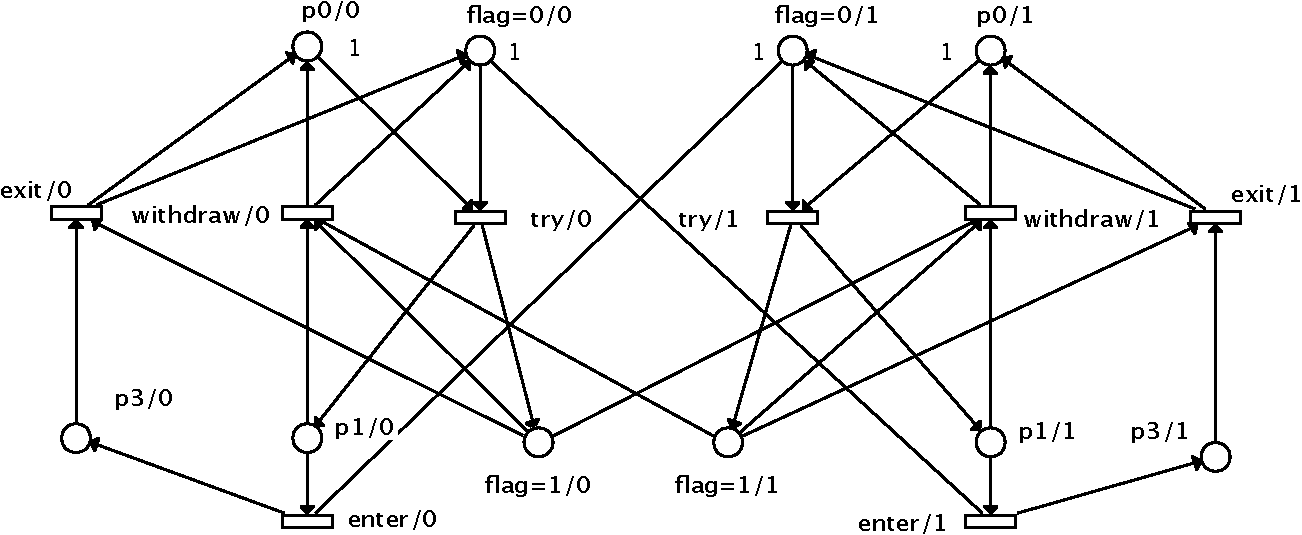
\includegraphics[scale=0.50]{fig/dekker2.pdf}
\caption{A variant of Dekker's mutual exclusion algorithm for two processes}
\label{f:dekker}
\end{figure}

\Cref{f:dekker} shows a c-net representing a variant of Dekker's mutual
exclusion algorithm for two processes, represented by numbers $0$ and~$1$
in the figure.
A process may fire \verb!try! and set a
\verb!flag! to signal intention to enter the critical section. 
It can then \verb!enter! the critical section \verb!p3!
if the other process is not trying.
Otherwise it may \verb!withdraw! its intention and clear the flag.  Read arcs
allow \verb!enter! and \verb!withdraw! to read the flag of the other process.

This c-net is distributed in the \verb!examples/! folder, included in the
precompiled binaries available in the tools's website, or the \verb!dist/!
folder generated after compilation.
The file in question is
\begin{verbatim}
examples/dekker/dek02.ll_net.
\end{verbatim}
For the purposes of this presentation, let us just give it a shorter name:
\begin{verbatim}
$ cp examples/dekker/dek02.ll_net dek02.ll_net
\end{verbatim}
This file, as any other c-net in the \verb!examples/! folder, is formated
in a simple modification of the PEP's \emph{low-level} Petri net
format, which will be described in \cref{s:formats}.
For historical reasons, this is the only input format of the \cunft{}.
The toolset comes, however, with
scripts to translate the output format of some graphical editors, like
\coloane\cite{Coloane} or PIPE2~v2.5\cite{BPK07}, see
\cref{s:producing} for more details.

\subsection{Constructing Unfoldings with Cunf}%{{{
\label{s:constructing}

Assume we wish to check if \verb!dek02.ll_net!
is deadlock-free, or whether mutual exclusion is guaranteed.
We first build its unfolding using \cunf,
and store it in the file \verb!u.cuf!:
\begin{verbatim}
$ cunf dek02.ll_net -i -s u.cuf
\end{verbatim}
By default \cunf outputs in \verb!CUF03! format
(documented in \cref{s:formats}).
A number of statistics about the computation of the unfolding
and the size and shape of the output are printed
just before the tool terminates.
We can distinguish the following lines:
\begin{verbatim}
[...]
histories            : 12
events               : 8
conditions           : 18
[...]
vector co(r) [avg]   : 5.25
vector rco(r) [avg]  : 0.50
[...]
pre-set(e) [avg]     : 1.75
context(e) [avg]     : 0.50
post-set(e) [avg]    : 1.75
cutoffs              : 6
[...]
\end{verbatim}
The first line above is the number of \emph{histories} generated by \cunf
(see\cite{BBCKRS12} for a definition), and gives a rough idea
of the size of the internal object \cunf had to build in order to produce the
unfolding.
The unfolding itself has the number of \emph{events} (transitions)
and \emph{conditions} (places)
reported in the next two lines.

\cunf's unfolding algorithm builds and maintains a \emph{concurrency relation}
that the tool internally needs for constructing the unfolding.
Explaining the purpose of this relation is out
of the scope of this manual (see\cite{BBCKRS12}).
It is, however, important to say that computation of this relation often takes
most of the time consumed by the tool.  In the line
\begin{verbatim}
co(r)   5.25
\end{verbatim}
\cunf reports that every element over which the relation is
defined was related to an average of 5.25 other elements.
This number gives an idea about the size of the concurrency relation.
In general, the higher it is the slower \cunf's unfolding algorithm advances.
See \cite[section 7]{BBCKRS12} for more details.

Next we see the average number of conditions in the 
preset, context, and postset of every event.  The last line reports
the number of cut-off (enriched) events present in the internal object
constructed by \cunf.

%}}}
\subsection{Deadlock and Coverability Analysis with Cna}%{{{
\label{s:deadlock}

After the construction of the unfolding, we can proceed to its analysis.
We use now \cna{} to ask, for instance, about the presence of deadlocks:
\begin{verbatim}
$ cna -d u.cuf
answer          : NO , the net is deadlock-free
clauses         : 52
event variables : 4
reductions      : bin 4-tree
sccs            : [(4, 4, 4, 4)]
variables       : 30
\end{verbatim}
Option \verb!-d! instructs \cna{} to look for deadlocks.
%\cna{} uses as input the contextual unfolding produced by \cunf{}.
By default, it will build and solve a propositional formula associated to the
unfolding, and will internally invoke \minisat to solve it.
If called with \verb!-n!, \cna will instead dump the formula and exit.

Option \verb!-c! checks for coverability, in this case, of places
\verb!p3/1! and \verb!p3/0!:
\begin{verbatim}
$ cna u.cuf -c 'p3/1' 'p3/0'
answer       : NO , no rechable marking covers 'p3/0' 'p3/1'
[...]
\end{verbatim}
Observe that \verb!p3/i! is marked iff process \verb!i! is in the critical
section.
We may also ask if it is possible to find one process trying to enter the
critical section while the other is already in, which is naturally possible:
\begin{verbatim}
$ cna u.cuf -c 'p1/0' 'p3/1'
answer          : YES, places 'p1/0' 'p3/1' are coverable
clauses         : 39
event variables : 4
reductions      : bin 4-tree
sccs            : [(4, 4, 4, 4)]
trace           : 'try/1:e0' 'enter/1:e3' 'try/0:e1'
variables       : 22
\end{verbatim}

The \verb!trace! indicates the firing sequence of the c-net (or the unfolding)
that makes possible to cover the requested places.
The lines labelled by \verb!clauses! and \verb!variables! inform about the
size of the SAT formula fed to \minisat.

Notice that in this example, the construction of the \verb!CUF03! file
is necessary only once, while \cna can be applied many times. For most
problems, the former step is the bottleneck whereas \cna works very fast
thanks to efficient SAT solving techniques. For cases where only one
coverability query is needed,
the option \verb!-t! of \cunf checks whether a given transition is
firable, and stops computing the unfolding if the answer is yes.
This can be used to check if the set of places in the preset of
a (intentionally inserted) transition is coverable.

Notice the line starting with \verb!reductions!.
\cna applies several optimizations to the SAT encoding it produces.
The word \verb!bin! means that it is using \emph{binary rankings} to
encode certain acyclicity constraint;
\verb!4-tree! says that \cna used
\textit{4-trees} to encode the absence of symmetric conflicts
(technical details in\cite{RS12,RS12rr}).
Run the tool without arguments to obtain a full list of all the
optimizations available, and information about them.
This information is available in \cref{s:cna}.
The effect of almost all them is described in\cite{RS12rr}.

%}}}
\subsection{More on Dekker's Algorithm}%{{{
\label{s:dekker}

How the unfolding grows as we add more processes to our model of the
Dekker's algorithm?

First, observe that when the 2-process example in \cref{f:dekker} is
generalized to $n$ processes, $\bigo{2^n}$ markings are
reachable in these c-nets --- for a net of size $\bigo{n^2}$.
Several instances of the protocol are distributed in the folder
\verb!examples/dekker/!.  We can easily run \cunf on some of them and retain
the unfolding size:
\begin{verbatim}
$ for i in 10 20 30 40 50; do
   cunf examples/dekker/dek$i.ll_net | grep events
done

events  120
events  440
events  960
events  1680
events  2600
\end{verbatim}
We see that the numbers roughly follow an square progression on the number of
processes involved, \ie, linear on the number of transitions of the c-net.

%while unfoldings of the equivalent Petri nets or
%the Place-Replication encodings\cite{BBC+12} are of size $\bigo{n^3}$.

%}}}
\subsection{Producing Graphics of C-nets and Unfoldings}%{{{
\label{s:seeing}

The \cunft{} is distributed with a number of scripts capable
of producing images depicting a c-net or an unfolding.
These scripts actually rely on the tool \verb!dot! from the Graphviz
project\cite{Graphviz} to actually produce the image.

Say that we want to \textit{see} the c-net \verb!dek02.ll_net! which we
unfolded in the previous sections.
We generate a \textit{dot} script out of the net, using the tool
\verb!pep2dot!, included in the \verb!src/! directory of the source code
(and also in the precompiled distribution):
\begin{verbatim}
$ src/pep2dot dek02.ll_net > dek02.dot
\end{verbatim}
Then use \verb!dot! tool, like this:
\begin{verbatim}
$ dot -T pdf < dek02.dot > dek02.pdf
\end{verbatim}
The file \verb!dek02.pdf! depicts the c-net.
Similarly, if we wish to see the unfolding, we could type:
\begin{verbatim}
$ scripts/cuf2pep.py < u.cuf > u.ll_net
$ src/pep2dot u.ll_net > u.dot
$ dot -T pdf < u.dot > u.pdf
\end{verbatim}
The first command has converted the \verb!cuf! file in to a
\verb!ll_net! file, and subsequent commands are like before.
The \verb!cuf2pep.py! script is also included in the precompiled
distribution.
The resulting PDF is shown in \cref{f:dek02unf}.
Regular arrows are in black, and read arcs are depicted in red.
The initially marked conditions are the four top ones,
and cut-off events have an asterisk in the name.

\begin{figure}[bt]
\centering
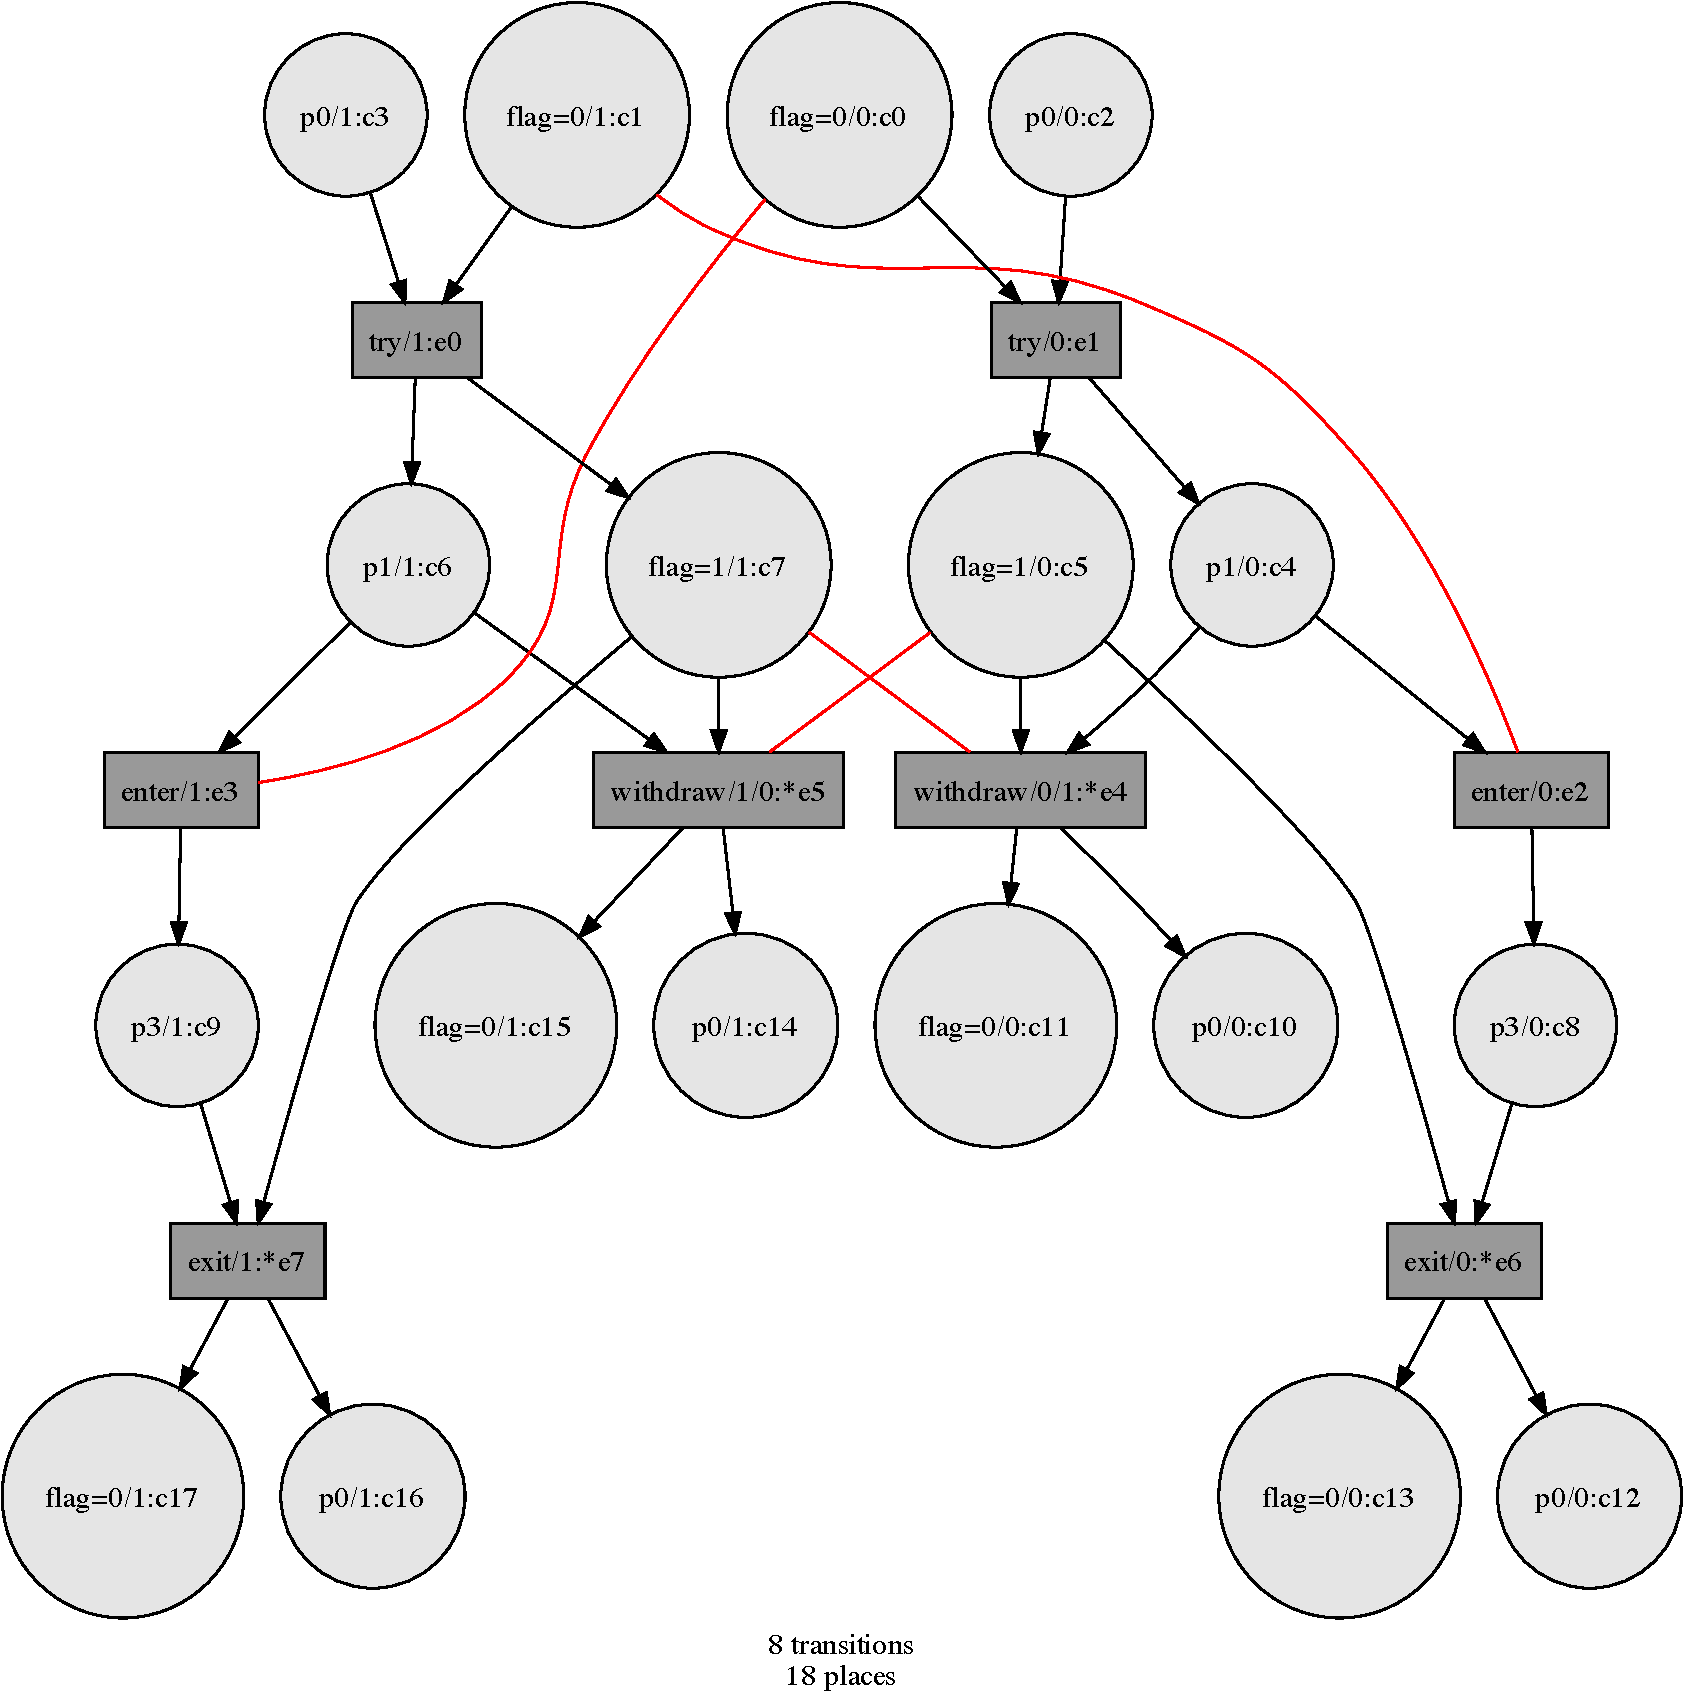
\includegraphics[scale=0.25]{fig/dek02-unf.pdf}
\caption{The unfolding of \cref{f:dekker}.}
\label{f:dek02unf}
\end{figure}

Actually, the \verb!make! machinery included in the source code already
knows how to produce PDF or even JPEG images of the c-nets
or unfoldings --- pretty much in the same way it knows how produce an
object file out of a C source file.
You just need to type \verb!make! followed from the desired file.
For instance, we can obtain a JPEG image of the c-net with:
\begin{verbatim}
$ make dek02.jpg
P2D dek02.ll_net
DOT dek02.dot
rm dek02.dot
\end{verbatim}
The tool \verb!make! reports that it first converts
the PEP \verb!ll_net! file into a \verb!dot! script (\verb!P2D!),
and then converts the \verb!dot! script into PDF (\verb!DOT!).
This will produce the file \verb!dek02.jpg!.

The same is true for building unfoldings.  To build the unfolding of a net
\verb!abc.ll_net! you just need to \textit{make} the file
\verb!abc.unf.cuf!:
\begin{verbatim}
$ make dist
$ make dist/examples/dijkstra/dij03.unf.cuf
UNF dist/examples/dijkstra/dij03.ll_net
time    0.013
mem     2
[...]
\end{verbatim}
Of course, more complex transformations can be achieved.  For instance, we
could generate a PDF depicting the unfolding of a c-net without
explicitly generating the \verb!cuf! file:
\begin{verbatim}
saiph:cunf$ make dist/examples/dijkstra/dij02.unf.pdf
UNF dist/examples/dijkstra/dij02.ll_net
time    0.001
mem     0
[...]
C2P dist/examples/dijkstra/dij02.unf.cuf
P2D dist/examples/dijkstra/dij02.unf.ll_net
DOT dist/examples/dijkstra/dij02.unf.dot
rm dist/examples/dijkstra/dij02.unf.ll_net
   dist/examples/dijkstra/dij02.unf.dot
   dist/examples/dijkstra/dij02.unf.cuf
\end{verbatim}
Observe that \verb!make! make is removing, in the last line, all
intermediate files it has generated --- because you did not ask for any of
them.  The file generated by the previous command is shown in
\cref{f:dij02unf}.

\begin{figure}[tb]
\centering
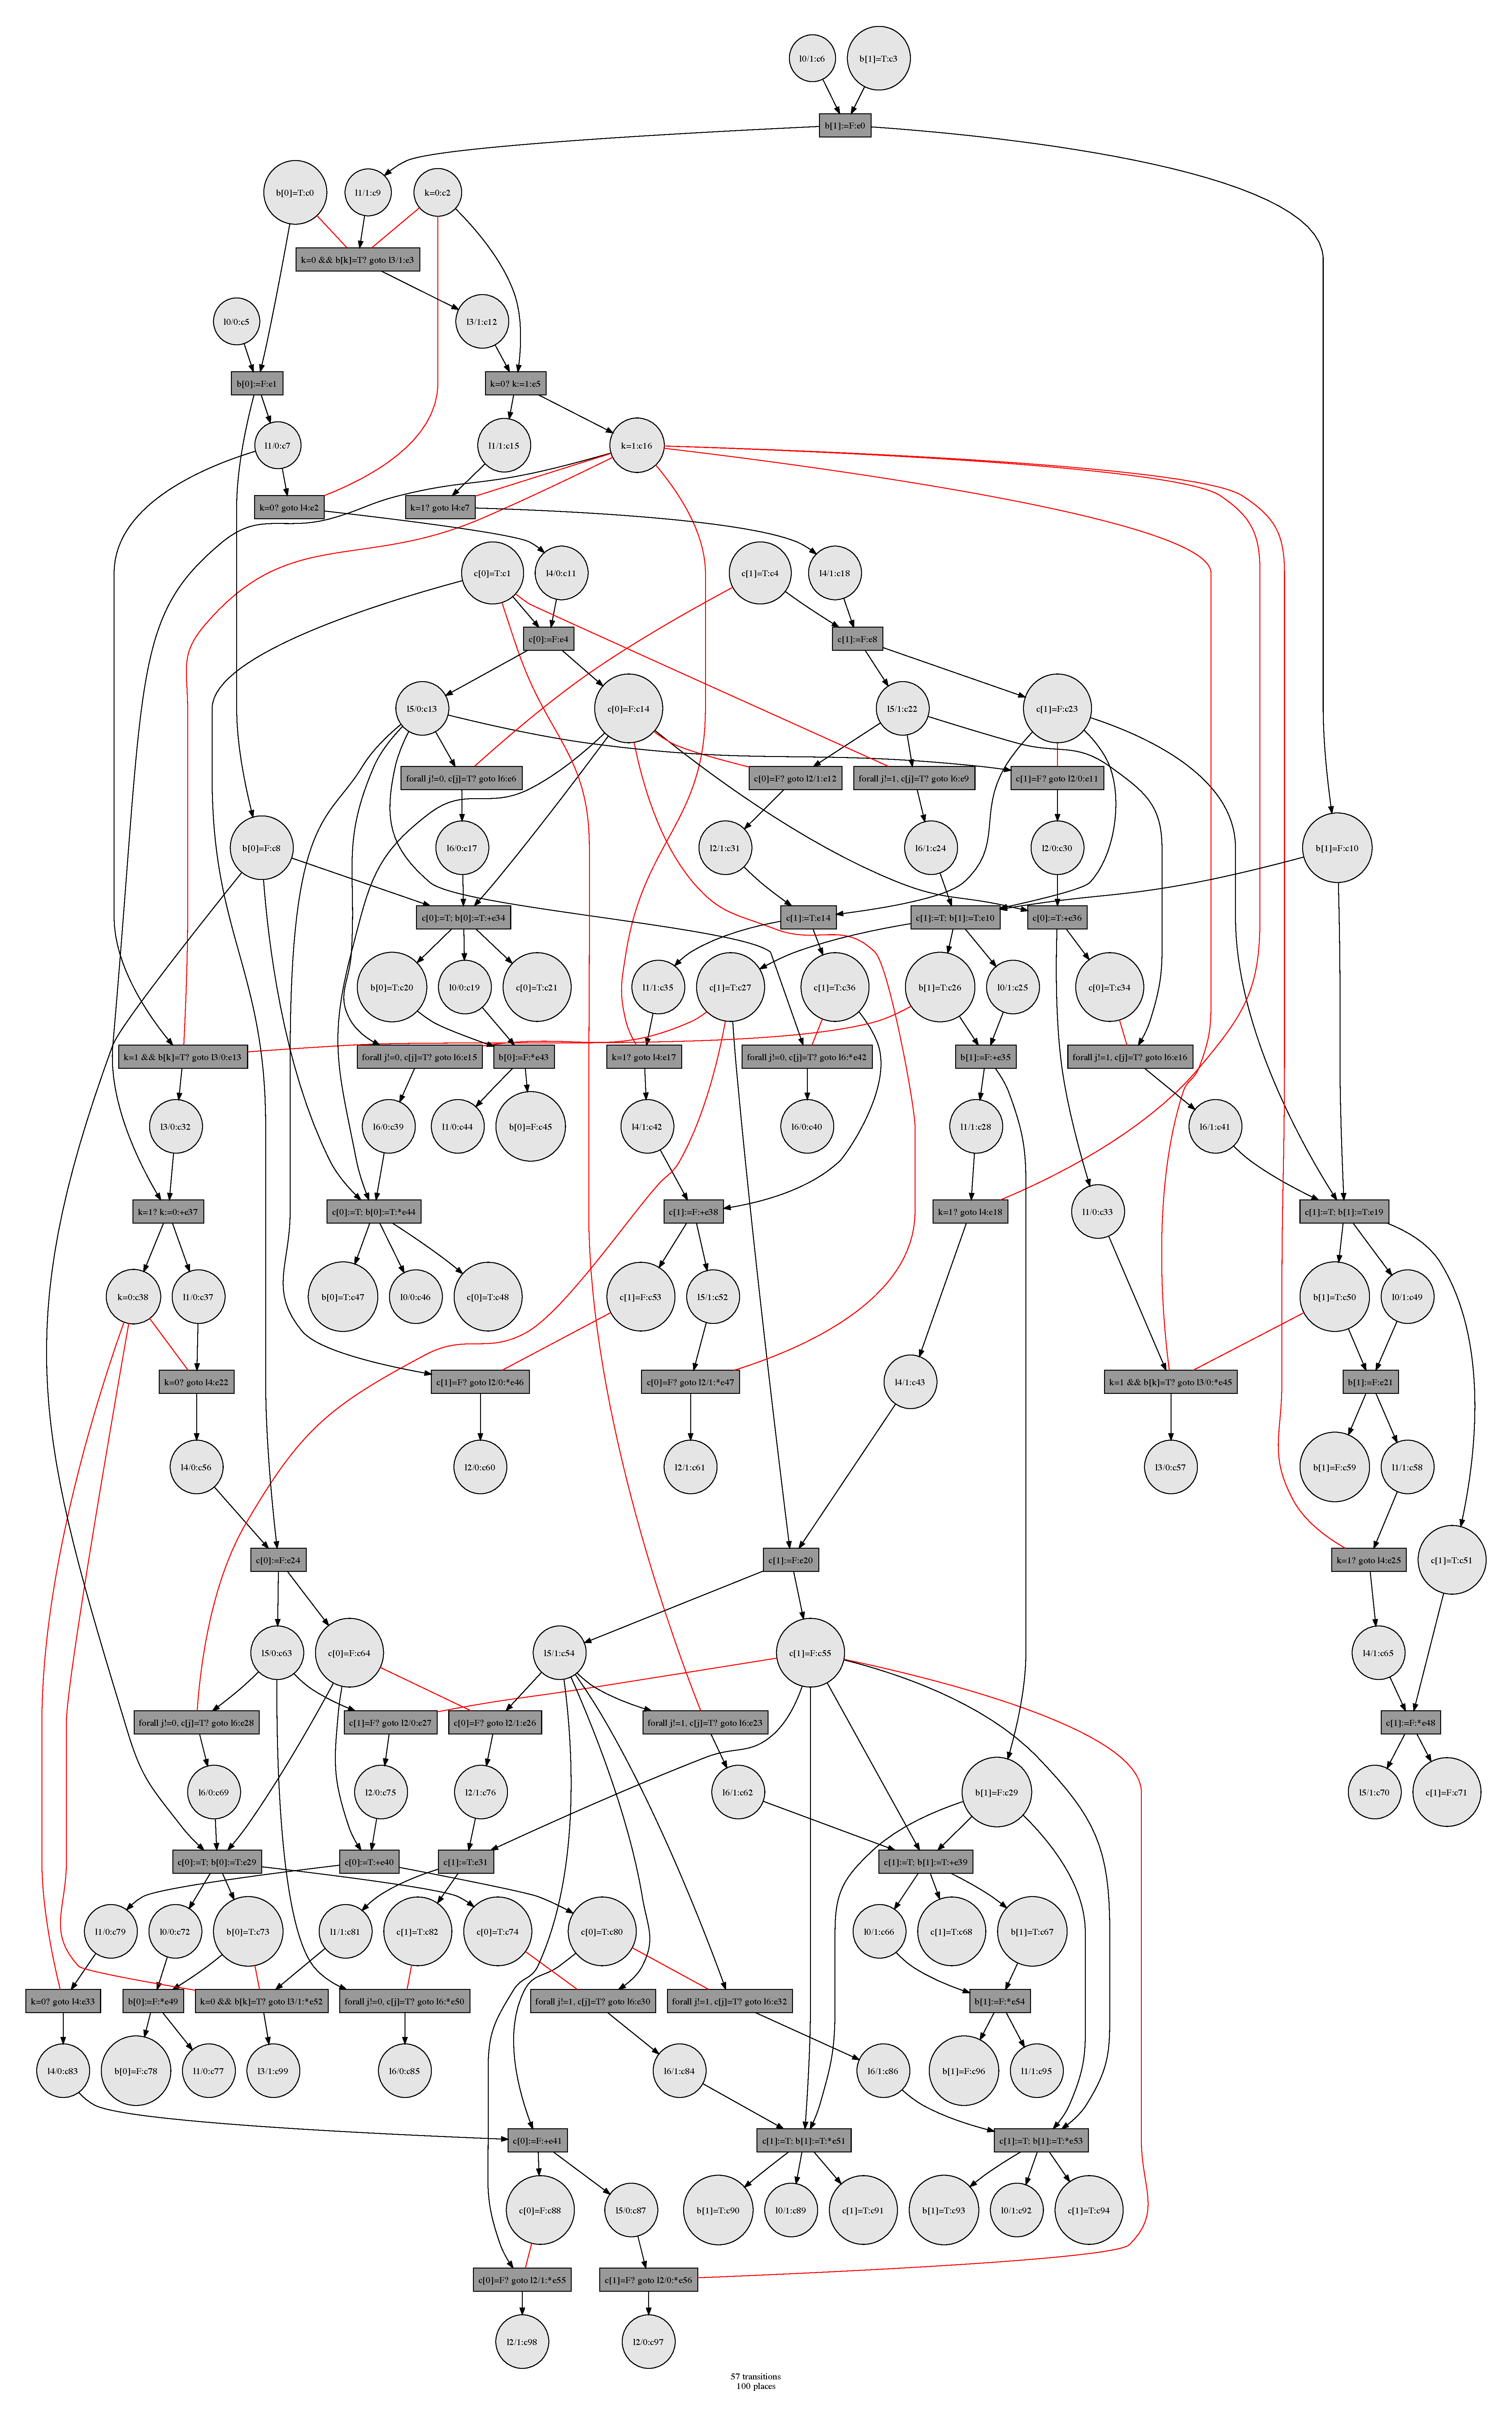
\includegraphics[scale=0.11]{fig/dij02-unf.pdf}
\caption{The unfolding of 
\cod{examples/dijkstra/dij02.ll\_net}.}
\label{f:dij02unf}
\end{figure}

If you wish to know other transformation rules \verb!make! knows, have a
look to the end of the file \verb!defs.mk!, located at the root of the
repository.

%}}}
\subsection{Finding More Examples}%{{{
\label{s:finding}

More examples are distributed in the \verb!examples/! folder of the package
containing the precompiled binaries or the (generated) \verb!dist/examples/!
folder in the source code:
\begin{description}
\item[\cod{examples/dijkstra/}]
  This folder contains c-nets modelling Dijkstra's mutual exclusion
  algorithm\cite{Dij65} for 2 up to 6 processes.
  They have been generated with the script \verb!scripts/mkdijkstra.py!,
  included in the source code (but not the bundle of precompiled binaries).

\item[\cod{examples/corbett/}]
  This is a superset of the of the popular benchmarks compiled by
  Corbett\cite{Cor96}.
  An short description of them can be found in\cite[\pp 29--31]{Kho03}
  
  The nets are distributed in four sub-folders.
  The folder \verb!cont/! contains contextual nets,
  and \verb!plain/! contains the plain encodings of the nets in
  \verb!cont/!.  Similarly, the folder \verb!pr/! contains the
  \emph{Place-Replication encoding}\cite{VSY98} of the same c-nets.
  The folder \verb!other/! contains ordinary Petri nets.
\end{description}

The folder \verb!scripts/! of the source code contains a number of scripts (all
them have names starting by \verb!mk!) to generate several families of nets,
other Dijkstra's or Dekker's mutual exclusion models.
This folder is \emph{not} distributed with the bundle of precompiled binaries.

%}}}%}}}
\iffalse%{{{
\section{Unfolding Construction and Analysis}
\label{s:cons}

In \cite{BCKS08}, Baldan et al. established theoretical foundations for
generating c-net unfoldings, whereas algorithmic details were spelt out
in \cite{BBC+12}. \cunf{} follows these lines. It inputs a
safe c-net (i.e.\ no place carries more than one token)
and outputs a complete unfolding prefix. A fundamental phenomenon present
in c-nets but not in Petri nets is \emph{asymmetric conflict} between an
event reading a token and an event consuming it, for instance
$t_2$ and $t_4$ in \rfig{examples}~(a).
%If $t_2$ and $t_4$ happen in the
%same run, then $t_2$ needs to happen before $t_4$. 
This phenomenon requires the c-net unfolding construction
to keep track of the so-called \emph{histories}. If $e$ is an event,
then 
a \emph{history} of $e$ is any set $H$ of events present in a run of
$\unf N$ that contains $e$ and such that any run that fires exactly all events
in $H$, fires $e$ last.
In (the unfolding of) \rfig{examples}~(a), the event labelled by $t_4$ has four
histories ($t_2$ and $t_3$ may or may not be included).
A pair $\tup{e, H}$ is called \emph{enriched event}. These changes could
not easily be accomodated by extending existing tools such as \mole{};
we therefore decided to implement a completely new tool. \cunf{} is written
in C and comprises roughly 4000 lines of code.

%The construction procedure works on a data structure that represents a prefix
%labelled with histories. It starts with a simple prefix,
%containing only the initial conditions $\widehat{m_0}$, and iteratively extends
%it with \emph{enriched events}, one at a time.
%Two challenging problems are involved in this construction.

\paragraph{Possible extensions.}
On average, \cunf{} spends more than 80\% of its time 
computing possible extensions,
i.e., the enriched events used to enlarge the prefix.
The problem is, given the current prefix $\ppref$ and one
transition $t$ of $N$, decide whether we can extend $\ppref$ with some enriched
event $\tup{e, H}$, where $f (e) = t$.  This is NP-complete and
requires solving a variant of the
coverability problem for a set of conditions $M$ where $f (M) = \pre t \cup
\cont t$.  \cunf{} achieves this by a \emph{concurrency relation} on
\emph{enriched conditions}\cite{RSB11a}, which is
efficiently updated while the prefix is extended.
The concurrency relation can be seen as a database that serves
to both solve coverability queries and update the relation itself.

\paragraph{Pruning.}
To keep the prefix finite, certain enriched events are marked as
\emph{cut-offs}, they are the pruning points of the otherwise potentially
infinite branches.
%If $\tup{e, H}$ is a cut-off, any $\tup{e', H'}$, where
%$H'$ \emph{includes} $H$, will be excluded.
%The cut-off criterion must allow
%\emph{all} reachable markings to be represented in the prefix, but shall,
%intuitively, prune unnecessary runs as soon as possible.
\cunf{} fixes an order $\prec$ on histories 
and extends the prefix only with $\prec$-minimal possible
extensions.
%This ensures that for a given enriched event $\tup{e, H}$, all
%enriched events $\tup{e', H'}$ with $H' \prec H$ are already present in the
%prefix.
$\tup{e, H}$ is a \emph{cut-off} if there exist some $\tup{e', H'}$ such
that $H' \prec H$ and $H$ reaches the same marking as $H'$: 
the future of $\tup{e, H}$ is unnecessary
because some \emph{smaller} enriched event, already included, leads to the same
markings.
Different variants of $\prec$ yield different prefix sizes and shapes.
\cunf{} implements the McMillan order\cite{McM92}, and a generalization of the
order $\prec_F$, see\cite{ERV02}.


as input, and produces as output
a complete (contextual) unfolding prefix of the input net.
The prefix is computed as follows.
First, the input net is loaded and represented in
memory by means of a graph-like data structure, in which, places and
transitions play the role of graph nodes and net arcs and read arcs play
the role of graph edges.  It subsequently searches for transitions with an
empty preset, producing a warning if one is found.  Note that Cunf does not
check whether the input net is 1-safe or not.

The unfolding procedure starts from a prefix consisting only on the initial
conditions, a copy of the initial marking of the input net.  A set $X$ of
events, so called \textit{possible extensions} of the prefix, is then
computed.  The prefix is subsequently extended by means of an iterative
procedure that appends one possible extension chosen from $X$ and updates
$X$ with the new possible extensions that arises from the last addition.
When this procedure stops, the prefix is written to disk and the tool
terminates, displaying by screen some information concerning the unfolding
computation and the output prefix itself.

The unfolding procedure stops, yielding a complete prefix, when either
there is no more possible extensions or all them are marked as
\textit{cutoffs}.  Cunf can additionally be instructed to stop and output
the unfolding prefix under other conditions.  The option \cod{-T}
specifies the name of a transition.  If provided, Cunf will stop once the
first possible extension labelled by that transition is found.  The tool
can also be requested to stop when the \textit{depth} of the history (see
\cref{compilation} for a definition) of every possible extension is greater
than a certain value, provided by the option \cod{-d}.

\fi%}}}
\section{Command-line Syntax}%{{{
\subsection{Cunf}%{{{

\cunf expects an optional list of command-line options followed by the
name of the input file to be provided as command-line arguments:
\begin{verbatim}
cunf [OPTIONS] NETFILE
\end{verbatim}
Run the tool without arguments to obtain the list of available options.
They are the next:

\begin{description}
\item[\cod{-t NAME}]
  Optional.  Stop the unfolding construction as soon as the transition
  \verb!NAME! is unfolded for the first time, and output the unfolding
  prefix currently built.  The prefix will include exactly one occurrence
  of the transition, if it has been found, or zero occurrences ---
  and it will be a \emph{marking-complete}, \cf \cite{BBCKRS12}.

\item[\cod{-d DEPTH}]
  Optional. \verb!DEPTH! is a natural number.
  Don't include in the unfolding prefix enriched events whose
  history has a depth greater or equal than \verb!DEPTH!.  The depth of a
  history $H$ is the maximum natural $n$ for which there exist events
  $e_1, \ldots, e_n$ in $H$
  such that $e_1 \nearrow e_2 \nearrow \ldots \nearrow e_n$,
  where $\nearrow$ is the \emph{asymmetric conflict relation}, as
  defined in\cite{BBCKRS12}.

\item[\cod{-o FILE}]
  Optional.  Write the unfolding prefix to the file \verb!FILE!.
  If not provided, \cunf will obtain the path to write the unfolding from
  the input file.  It will strip the string \verb!ll_net! from the
  \verb!INPUT! file and will concatenate the string \verb!unf.dot!.

\item[\cod{-f FORMAT}]
  Optional. \verb!FORMAT! shall be one of
  \verb!cuf!,
  \verb!dot!, or
  \verb!fancy!.
  See \cref{s:oformat}.
\end{description}

%}}}
\subsection{Cna{}}%{{{
\label{s:cna}

Run \cna without arguments to obtain help about its command-line syntax.
The tool expects a mandatory \verb!CUF! file and an optional
\verb!OUTFILE! where it will write its textual output (standard output if
not given):

\begin{verbatim}
cna [CUF] [OUTFILE] [OPTIONS]
\end{verbatim}

Here is the list of \verb!OPTIONS! it accepts:

\begin{description}
\item[\cod{-h}, \cod{--help}]
  Show a help message and exit.

\item[\cod{-d}, \cod{--deadlock}]
  Optional.  Default: no.
  Tell whether or not a deadlocked marking is reachable.
  At least one of \cod{-d} or \cod{-c} must be given.

\item[\cod{-c PLACE [PLACE ...]}, \cod{--cover PLACE [PLACE ...]}]
  Optional.  Default: no.
  Tell whether or not the list of \verb!PLACE!s are coverable.
  You may consider quoting place names if they contain spaces
  At least one of \cod{-d} or \cod{-c} must be given.

\item[\cod{-r REDUC [REDUC ...]}, \cod{--reduce REDUC [REDUC ...]}]
  Default: \cod{4-tree bin}.
  Use \verb!REDUC!tions of the propositional formula generated by the tool
  that improve running time of the SAT
  solver.  The following options are available:
  \begin{description}
  \item[\cod{k-tree}]
    (where 1 $<$ \verb!k! $<$ 10)  Use $k$-trees to implement the
    at-most-one constraints in the encoding of symmetric conflicts.
    If none of the options `\cod{seq}', `\cod{log}', or `\cod{pair}' is
    present, \cod{4-tree} will be used.
  \item[\cod{seq}]
    Use the sequential encoding of\cite{Sinz05} for symmetric conflicts.
  \item[\cod{log}]
    Use the logaritmic encoding of\cite{Frisch05} for symmetric conflicts.
  \item[\cod{pair}]
    Use pairwise encoding for symmetric conflicts.
  \item[\cod{stb}]
    Use elimination of stubborn events, see\cite{RS12rr} for a detailed,
    technical description of the optimization.
  \item[\cod{sub}]
    Reduce the \emph{symmetric} and \emph{disabled} constraints to certain
    maximal sets.
  \item[\cod{nocy}]
    Do not produce constraints to check for cycles in the asymmetric
    conflict relation.
  \item[\cod{bin}]
    Generate acyclicity constraints using ranks with binary encoding,
    see\cite{CGS09}. 
    If none of the options `\cod{nocy}', `\cod{trans}', or `\cod{unary}' is
    present, `\cod{bin}' will be used.
  \item[\cod{unary}]
    Generate acyclicity constraints using ranks with unary encoding.
  \item[\cod{trans}]
    Generate acyclicity constraints encoding transitive closure.
  \item[\cod{sccred}]
    Reduce the SCCs before generating the acyclicity constraints.
  \end{description}

\item[\cod{-n FILE}, \cod{--dont-solve FILE}]
  Dump the propositional formula to \verb!FILE! and exit, instead of
  running the solver and displaying the result.

%\item[\cod{-v}, \cod{--verbose}]
%  Causes the tool to print debugging messages.  Not implemented.
\end{description}

%}}}%}}}
\section{File Formats}%{{{
\label{s:formats}

\subsection{The \cod{ll\_net} Format}%{{{
\label{s:iformat}

\cunf accepts a c-net as input, represented in a slightly modified version
of the PEP's low-level format.  We describe here this modification.  We
assume the reader is familiar with the PEP's low-level format\cite{PEP,B98}.

The input file should be formated in the low-level net syntax extended with
one additional section, which specifies the context relation.  The new
section contains a list of read arcs, each one specified in the same way as
either the place-transition arcs in section \cod{PT} or the
transition-place arcs in section \cod{TP}.  The new section is headed by the
keyword \cod{RA}, standing for Read Arcs.  

Sections in the low-level net format must be placed in certain order.  The
new \cod{RA} section must appear after the section \cod{TP} (transition to
place arcs) and before the (optional) section \cod{PTP} (phantom transition
to place arcs).  \Cref{f:modified.low} shows an example, together with the
graphical representation of the c-net.

\begin{figure}[bth]
\begin{center}
\begin{minipage}{.3\textwidth}
\footnotesize
\begin{verbatim}
PEP
PetriBox
FORMAT_N2
PL
"P0"M1
"P1"M1
"P2"
"P3"
"P4"
"P5"
TR
"T0"
"T1"
"T2"
"T3"
TP
1<3
2<4
3<5
4<6
PT
1>1
2>2
3>3
3>4
4>4
RA
2<1
\end{verbatim}
\end{minipage}
\begin{minipage}{5cm}
\includegraphics{fig/modified-low.fig}
\end{minipage}
\end{center}
\caption{Example of the \cod{ll\_net} format with read arcs,
and graphical representation of the encoded c-net.}
\label{f:modified.low}
\end{figure}
%}}}
\subsection{Unfolding Formats}%{{{
\label{s:oformat}

\cunf can write its output, the unfolding of the input c-net,
in several formats. By default, it will write a \verb!cuf! file, but
other formats can be selected with the option \verb!-f!:
\begin{description}
\item[\cod{dot}]
  For historical reasons, \cunf is able to write \verb!dot!  scripts,
  suitable for the \verb!dot! tool.
  Scripts to produce \verb!dot! input out any \verb!cuf! or file are
  included in the source and precompiled distributions.

\item[\cod{fancy}]
  This also produces a \verb!dot! file, but every event in the resulting
  graphical representation of the unfolding is annotated by the histories
  that \cunf had to construct.  This is right now the only way of
  extracting information about the history-enriched unfolding prefix that
  \cunf constructs --- apart from compiling the tool with
  \verb!CONFIG_DEBUG! and parsing the debugging output.

\item[\cod{cuf}]
 The default output format, called \verb!CUF03!, is binary and similar to
 the MCI format of PEP.  C and Python code for dealing with \verb!CUF03!
 files is available in the repository.
 
 The standard reference defining the \verb!CUF03! format is the comment in
 the the line 263 of the file
\begin{verbatim}
src/output.c,
\end{verbatim}
 just before the function \verb!write_cuf!.  All technical
 details of the file format are explained there.
\end{description}

%}}}%}}}
\section{Producing Input for Cunf}%{{{
\label{s:producing}

Most of the c-nets on which the \cunft{} has been used has been
generated programmatically.  It is the case, for instance, of the
\verb!dekNN.ll_net! nets in \cref{s:getting}.

Sometimes it is interesting, however, to draw a c-net and perform some
analysis on it.
There is currently no graphical user interface in the \cunft{}, and there is
no plan for it to be available in the future.
The \cunft{} is however integrated in the \cosyverif\cite{Cosyverif} tool,
which includes a graphical interface and which will internally invoke the
\cunft{} in several mouse clicks.
There is also plans to include the \cunft{} as a verification engine
of \tapaal\cite{DJJJMS12}.

\subsection{Graphically}%{{{
\label{s:graphically}

A simple way of producing c-nets for \cunf is
using the \coloane graphical editor\cite{Coloane}.  This is the same editor
used in the Cosyverify tool, but can be installed as an stand-alone
program.  Once you have edited your c-net in \coloane, see \cref{f:coloane}
(observe that you can also introduce read arcs), right-click on the model
name in the \textit{Projet Explorer} window, and then click on
\textit{Export}.  Export the c-net in GRML format.\footnote{The dialog
could incorrectly display GML, instead of GRML.}

\begin{figure}[bth]
\hspace{-4em}
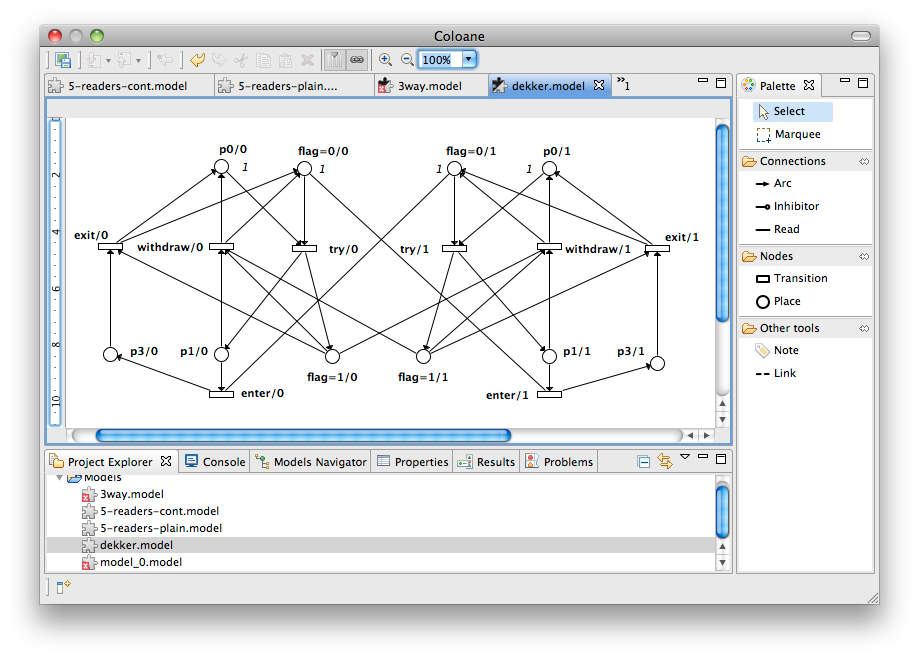
\includegraphics[scale=0.4]{fig/coloane.png}
\caption{The \coloane graphical editor can export c-nets for the \cunft{}.}
\label{f:coloane}
\end{figure}

Once your file, say \verb!net.grml! (the extension is important),
is in GRML format, use the script
\verb!grml2pep.py! to convert the file into
\verb!ll_net! format.  If you read \cref{s:seeing}, you will be unsurprised
to know that the \verb!make! machinery of the \cunft{} sources
also knows about GRML files.  You can, alternatively, type:
\begin{verbatim}
$ make net.ll_net
\end{verbatim}
or even directly
\begin{verbatim}
$ make net.unf.cuf
\end{verbatim}

%}}}
\subsection{Programmatically}%{{{
\label{s:program}

A Python module for reading and writing a number of c-net and Petri net
formats is distributed with the \cunft{}.
\cna actually uses it to read \verb!cuf! files and many scripts in the
\verb!scripts/! folder of the sources use it to carry out various operations.
All \verb!scripts/mk*! scripts use this module, \cf \cref{s:finding}.

We briefly illustrate its use with a simple example.  The following code
produces the c-net in \cref{f:ptnet}

\begin{verbatim}
import sys
import ptnet

# creates the net object
n = ptnet.net.Net ()

# creates three places, two initially marked
p1 = n.place_add ('p1', 1)
p2 = n.place_add ('p2', 1)
p3 = n.place_add ('p3')

# and two transitions
t1 = n.trans_add ('t1')
t2 = n.trans_add ('t2')

# sets arrows and read arcs
t1.cont_add (p2)
t1.pre_add (p1)
t2.pre_add (p1)
t1.post_add (p3)
t2.post_add (p3)

# writes the c-net in 'pep' format,
# see source code to know about other formats
n.write (sys.stdout, 'pep')
\end{verbatim}

\begin{figure}[bth]
\centering
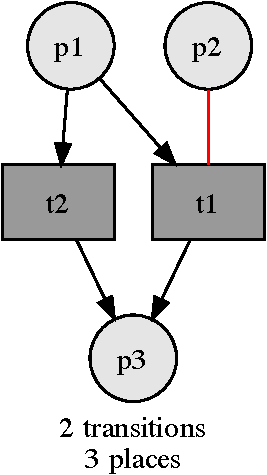
\includegraphics[scale=0.5]{fig/ptnet.pdf}
\caption{A c-net programmatically produced with the \cod{ptnet} Python
module.}
\label{f:ptnet}
\end{figure}

%}}}%}}}

%\renewcommand{\refname}{\vspace{-2em}}
\bibliographystyle{plain}
\bibliography{refs}

\end{document}

% vim: set efm=%f\:%l%.%m,%f\:%m:
